\documentclass[11pt]{beamer}
% \usetheme{Boadilla}
  \usetheme{default}


% acronyms for text or math mode
\newcommand {\ccast} {\mbox{\small CCAST}}
\newcommand {\cris} {\mbox{\small CrIS}}

\newcommand {\airs} {\mbox{\small AIRS}}
\newcommand {\iasi} {\mbox{\small IASI}}
\newcommand {\idps} {\mbox{\small IDPS}}
\newcommand {\nasa} {\mbox{\small NASA}}
\newcommand {\noaa} {\mbox{\small NOAA}}
\newcommand {\nstar} {\mbox{\small STAR}}
\newcommand {\umbc} {\mbox{\small UMBC}}
\newcommand {\uw}   {\mbox{\small UW}}

\newcommand {\fft}  {\mbox{\small FFT}}
\newcommand {\ifft} {\mbox{\small IFFT}}
\newcommand {\fir}  {\mbox{\small FIR}}
\newcommand {\fov}  {\mbox{\small FOV}}
\newcommand {\for}  {\mbox{\small FOR}}
\newcommand {\ict}  {\mbox{\small ICT}}
\newcommand {\ils}  {\mbox{\small ILS}}
\newcommand {\igm}  {\mbox{\small IGM}}
\newcommand {\opd}  {\mbox{\small OPD}}
\newcommand {\rms}  {\mbox{\small RMS}}
\newcommand {\zpd}  {\mbox{\small ZPD}}
\newcommand {\ppm}  {\mbox{\small PPM}}
\newcommand {\srf}  {\mbox{\small SRF}}

\newcommand {\ES} {\mbox{\small ES}}
\newcommand {\SP} {\mbox{\small SP}}
\newcommand {\IT} {\mbox{\small IT}}
\newcommand {\SA} {\mbox{\small SA}}

\newcommand {\ET} {\mbox{\small ET}}
\newcommand {\FT} {\mbox{\small FT}}

% abbreviations, mainly for math mode
\newcommand {\real} {\mbox{real}}
\newcommand {\imag} {\mbox{imag}}
\newcommand {\atan} {\mbox{atan}}
\newcommand {\obs}  {\mbox{obs}}
\newcommand {\calc} {\mbox{calc}}
\newcommand {\sinc} {\mbox{sinc}}
\newcommand {\psinc} {\mbox{psinc}}
\newcommand {\std} {\mbox{std}}

% symbols, for math mode only
\newcommand {\wnum} {\mbox{cm$^{-1}$}}
\newcommand {\lmax} {L_{\mbox{\tiny max}}}
\newcommand {\vmax} {V_{\mbox{\tiny max}}}

\newcommand {\tauobs} {\tau_{\mbox{\tiny obs}}}
\newcommand {\taucal} {\tau_{\mbox{\tiny calc}}}
\newcommand {\Vdc}  {V_{\mbox{\tiny DC}}}

\newcommand {\rIT} {r_{\mbox{\tiny\textsc{ict}}}}
\newcommand {\rES} {r_{\mbox{\tiny\textsc{es}}}}
\newcommand {\robs} {r_{\mbox{\tiny obs}}}

\newcommand {\rITobs} {r_{\mbox{\tiny\textsc{ict}}}^{\mbox{\tiny obs}}}
\newcommand {\rITcal} {r_{\mbox{\tiny\textsc{ict}}}^{\mbox{\tiny cal}}}

\newcommand {\ITmean} {\langle\mbox{\small IT}\rangle}
\newcommand {\SPmean} {\langle\mbox{\small SP}\rangle}


\title{ccast intro and overview}
\author{H.~E.~Motteler}
\institute{
  UMBC Atmospheric Spectroscopy Lab \\
  Joint Center for Earth Systems Technology \\
}
\date{\today}
\begin{document}

%----------- slide --------------------------------------------------%
\begin{frame}[plain]
\titlepage
\end{frame}
%----------- slide --------------------------------------------------%
\begin{frame}
\frametitle{introduction}

\ccast\ takes level zero data from the Cross-track Infrared Sounder
(CrIS), a Fourier transform spectrometer on the Suomi NPP and JPSS
weather satellites, and produce high-quality calibrated radiances.
It is written primarily in Matlab, allowing for easy interaction,
modification, and data visualization.  We give a brief overview of
the design, implementation, and use.

\hspace{2cm}

The authors of the \umbc\ \ccast\ are Howard E.~Motteler, David Tobin,
L.~Larrabee Strow, and Dan Mooney, with interferometric parameters
in spreadsheet form from Joe Predina.

\hspace{2cm}

\ccast\ is available as a GitHub public repository and is distributed
under the terms of the GNU GPL v3.

\end{frame}
%----------- slide --------------------------------------------------%
\begin{frame}
\frametitle{history}

\begin{itemize}
  \item \ccast\ started as a collaboration between \umbc\ and
    \uw\ in fall 2010, with major components from the 2007-2008 FM1
    bench and TVAC tests.

  \item H.~Motteler wrote the L1a processing, starting with Dan
    Mooney's RDR reader, and L.~Strow, Dave Tobin, and H.~Motteler
    all collaborated on the L1b 

  \item this forked into a \uw\ version with Fred Nagel's geo that
    got first light, and a \umbc\ version with \noaa\ geo that got
    the first high res obs a month later.

  \item in the summer of 2012 H.~Motteler updated the UW code to 
    run in the \umbc\ environment, and for some time maintained both
    versions while continuing to develop the \umbc\ branch.

  \item major portions of the \uw\ branch, including \ict\ modeling
    and the non-linearity correction, were updated and merged into
    the \umbc\ branch.
\end{itemize}


\end{frame}
%----------- slide --------------------------------------------------%
\begin{frame}
\frametitle{preprocessing}

\begin{center}
  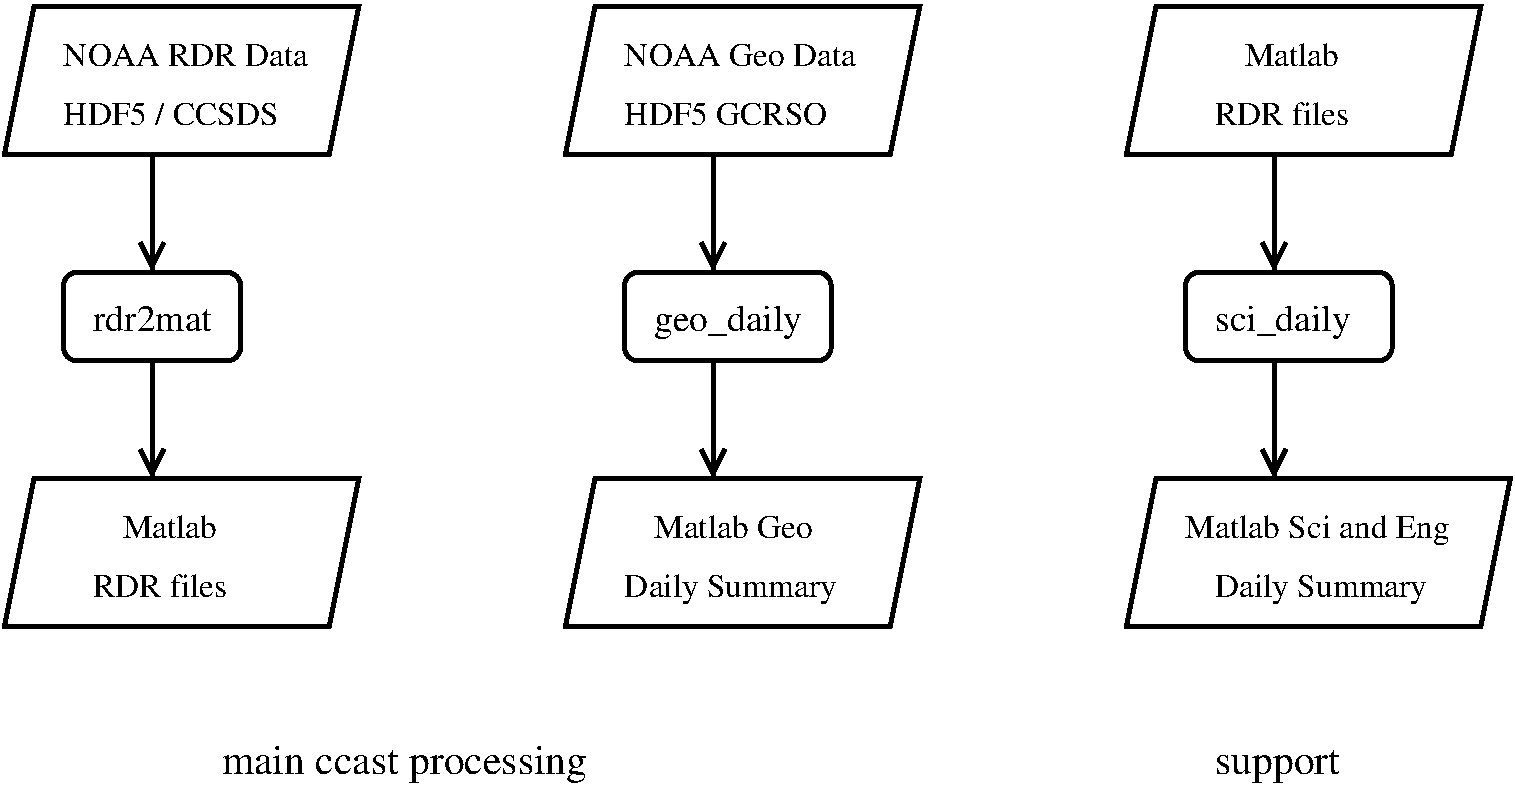
\includegraphics[scale=0.4]{figures/prepro.pdf}
\end{center}

\end{frame}
%----------- slide --------------------------------------------------%
\begin{frame}
\frametitle{preprocessing}

\ccast\ processing is done in two passes---the first takes HDF and
CCSDS data to Matlab files, and the second takes the Matlab files to
calibrated radiances.  The preprocessing is done by ccast\_prepro.
The main steps are

\begin{itemize}
  \item rdr2mat -- read \noaa\ RDR files (CCSDS level 0 data with an
    HDF-5 wrapper) and produce Matlab RDR files, our working level~0
    format.

  \item geo\_daily -- read \noaa\ GCRSO HDF-5 geo files and produce a
    daily abstract of CrIS geo data, as matlab files.

  \item sci\_daily -- read Matlab RDR files and produce a daily
    abstract of ``science'' (8~second) and ``engineering''
    (4~minute) support data, as matlab files.

\end{itemize}

\end{frame}
%----------- slide --------------------------------------------------%
\begin{frame}
\frametitle{main processing}

\begin{center}
  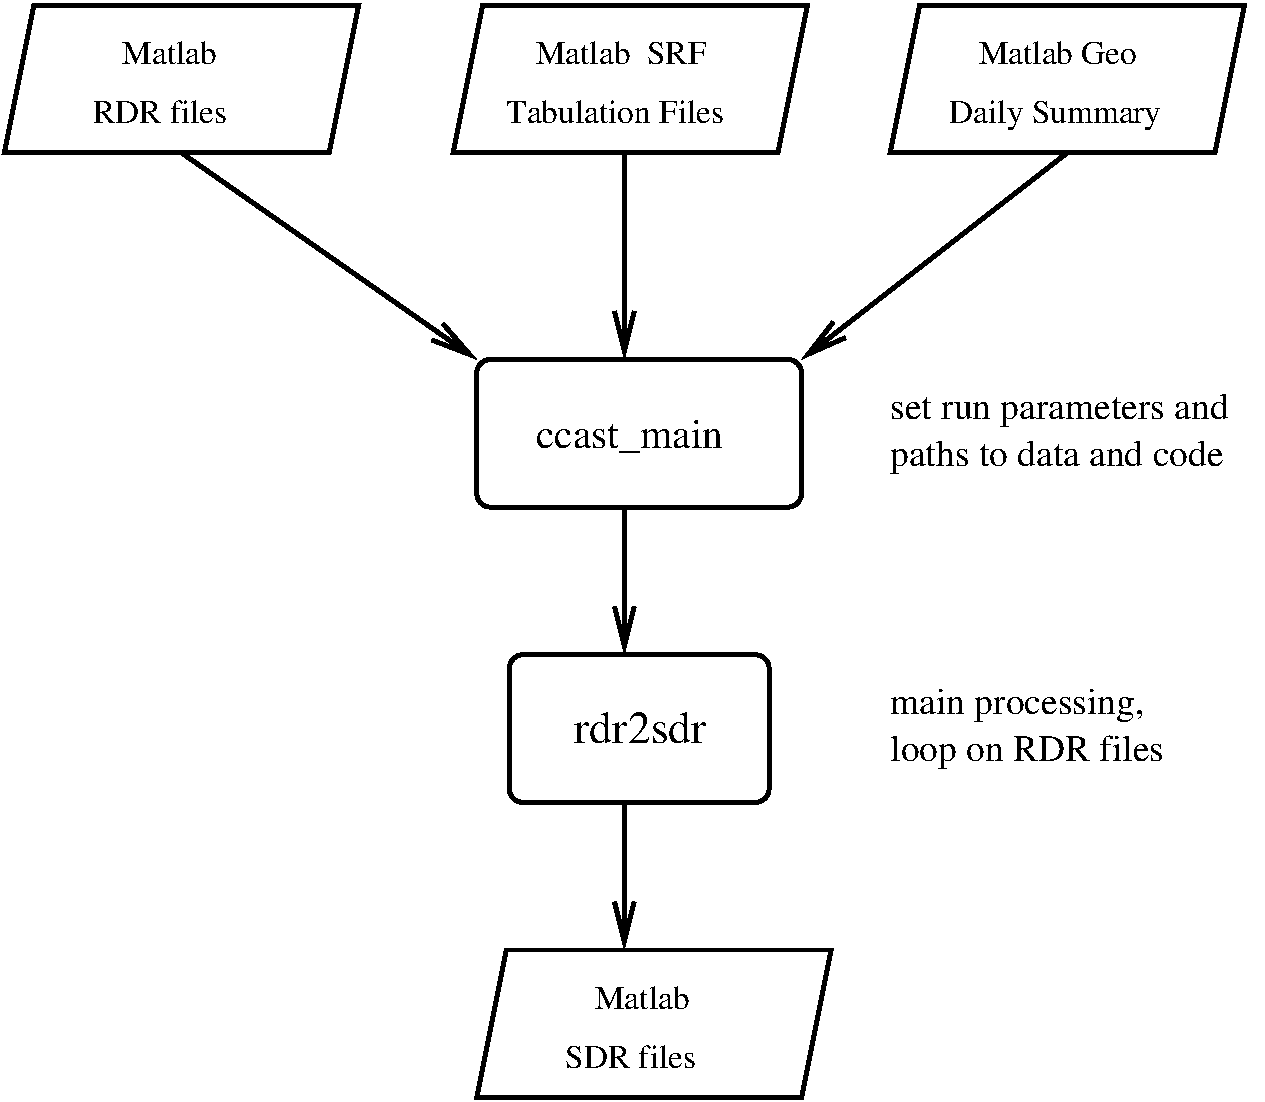
\includegraphics[scale=0.4]{figures/mainpro.pdf}
\end{center}

\end{frame}
%----------- slide --------------------------------------------------%
\begin{frame}
\frametitle{main processing}

ccast\_main sets parameters and paths and calls rdr2sdr, which 
loops on Matlab RDR files, typically one day per call.  The main
processing steps in rdr2sdr are

\begin{itemize}
  \item checkRDR -- validate and order the RDR data
  \item scipack  -- process sci and eng packet data
  \item inst\_params -- user and sensor grid parameters
  \item igm2spec -- take interferograms to count spectra
  \item scanorder -- group data into scans
  \item geo\_match  -- match GCRSO and RDR scans
  \item movavg\_app -- calculate moving averages
  \item calmain  -- radiometric and spectral calibration
\end{itemize}

\end{frame}
%----------- slide --------------------------------------------------%
\begin{frame}
\frametitle{design notes}

Some high-level design choices reflect past expedience and
incremental development.

\begin{itemize}
  \item there is no granule structure, data is organized as
    sets of scans

  \item the \noaa\ RDR files can start and stop at any field of
    regard (FOR), and the output SDR files follow this organization.

  \item the translation to count spectra should be done later, right
    before taking moving averages

  \item there is no explicit quality control for the final
    calibrated product.  There is extensive low-level data QC, and
    most output and working arrays are initialized with NaNs as a
    sanity check on processing

  \item the use of the geo summary files was originally meant to be
    temporary; the geo\_match procedure could read the GCRSO files
    directly

\end{itemize}

\end{frame}
%----------- slide --------------------------------------------------%
\begin{frame}
\frametitle{performance}

\begin{itemize} 
  \item \ccast\ produces high-quality calibrated radiances.
    Although it borrows significantly from the NOAA ATBD, key
    features such as the ILS, SA interpolation, and the form of the
    calibration equation were developed independently and in some
    cases have been adopted by other groups.

  \item runtime performance is very good.  Running as a single task
    rdr2sdr processes 60-scan files at a rate of slightly less than
    one file per minute

  \item reliability is very good.  We have repeatedly reprocessed
    all data from mission start with no problems.

\end{itemize} 

\end{frame}
%----------- slide --------------------------------------------------%
\begin{frame}
\frametitle{to-do list}

\begin{itemize}
  \item continue to improve the documentation.

  \item regularize the output and expand the draft matlab\_sdr.txt
    into more user-friendly data definitions

  \item vectorize the non-linearity correction and set non-linearity
    parameters in inst\_params.

  \item add file spanning moving averages.  This was on hold pending
    possible lower level regularization or the addition of a granule
    structure.

  \item add some QC for the final calibrated product, including the
    residual complex component from the calibrated radiances

  \item consider switching to a faster RDR reader.  Dan Mooney's
    reader (with some local mods) has been very reliable, but is
    idiosyncratic and slow relative to the rest of the processing.

\end{itemize}

\end{frame}
%----------- slide --------------------------------------------------%
\begin{frame}
\frametitle{getting started}

\begin{itemize} 
   \item to download the ccast repo \\ 
     \hspace{10pt} git clone https://github.com/strow/ccast.git
   \item to update a local copy of the ccast repo \\ 
     \hspace{10pt} git pull origin master
   \item see ccast/README for info on installation and testing, and
     for URLS to test data and sample SRF tabulations
   \item see ccast/doc for
     \begin{itemize}
       \item ccast\_intro.pdf -- this document
       \item ccast\_eqns.pdf -- ILS and main calibration equations
       \item matlab\_sdr.txt -- output data format and fields
       \item finterp.pdf -- notes on Fourier interpolation
     \end{itemize} 
\end{itemize} 

\end{frame}
%----------- slide --------------------------------------------------%
\end{document}
